\subsection{Generación de señalamiento paso a paso}

Al ejecutar el RNA, primero detectará todos los \textit{netElements}, sus coordenadas iniciales y finales en la topología, y el sentido en el que fueron definidas. El resultado obtenido se muestra en el Cóodigo \ref{lst:EJ4_1}.

\begin{lstlisting}[language = {}, tabsize=4, basicstyle=\footnotesize\ttfamily, showspaces=false, showstringspaces=false, caption = Detección de \textit{netElements} por parte del RNA , label = {lst:EJ4_1}]
	###### Starting Railway Network Analyzer #####
	Reading .railML file
	Creating railML object
	Analyzing railML object
	Analyzing graph
	ne991 [-1064, 0] [-2322, 0] <<
	ne61 [4350, 0] [4804, 250] >> 
	ne63 [4350, 0] [5763, 0] >>
	ne65 [7444, 0] [5763, 0] <<
	ne910 [11254, 0] [11822, 250] >>
	ne912 [11254, 0] [13111, 0] >>
	ne114 [15670, 0] [14482, 0] <<
	ne288 [-1064, 0] [-741, 250] >>
	ne290 [-1064, 0] [-211, 0] >>
	ne292 [864, 0] [-211, 0] <<
	ne295 [-741, 250] [457, 250] >>
	ne297 [457, 250] [720, 250] >>
	ne377 [350, -200] [-92, -200] <<
	ne384 [457, 250] [-104, 450] <<
	ne400 [6904, 250] [7194, 250] >>
	ne404 [4804, 250] [6904, 250] >>
	ne407 [6904, 250] [5855, 500] <<
	ne421 [6454, -259] [5915, -259] <<
	ne450 [14722, 250] [14232, 250] <<
	ne465 [13772, -259] [13263, -259] <<
	ne98 [1573, 0] [3687, 0] >>
	ne99 [3687, 0] [4350, 0] >>
	ne100 [8372, 0] [10727, 0] >>
	ne101 [10727, 0] [11254, 0] >>
	ne102 [15670, 0] [18172, 0] >>
	ne104 [-509, 630] [-104, 450] >>
	ne110 [-104, 450] [-741, 250] <<
	ne111 [-211, 0] [-92, -200] >>
	ne113 [-92, -200] [-749, -200] <<
	ne122 [5304, 759] [5855, 500] >>
	ne123 [5855, 500] [4804, 250] <<
	ne124 [5763, 0] [5915, -259] >>
	ne126 [5915, -259] [5354, -259] <<
	ne127 [14232, 250] [13022, 500] <<
	ne129 [14232, 250] [14482, 0] >>
	ne130 [14232, 250] [11822, 250] <<
	ne131 [13111, 0] [13263, -259] >>
	ne132 [13111, 0] [14482, 0] >>
	ne133 [13263, -259] [12722, -259] <<
	ne134 [12452, 810] [13022, 500] >>
	ne135 [13022, 500] [11822, 250] <<
	ne992 [7444, 0] [8372, 0] >>
	ne993 [7194, 250] [7504, 250] >>
	ne994 [7444, 0] [7194, 250] <<
	ne995 [720, 250] [1020, 250] >>
	ne996 [864, 0] [1573, 0] >>
	ne997 [720, 250] [864, 0] >>
	The network is connected
\end{lstlisting}

Por ejemplo, el \textit{netElement} ne995 inicia en la coordenada (720;250) y finaliza en la coordenada (1020;250). El símbolo $>>$ indica que ne1 se encuentra definido de izquierda a derecha, ya que la componente x de la coordenada final es mayor a la de la coordenada inicial, teniendo la misma componente y. Además, se puede comprobar que la lista obtenida en consistente con la Figura \ref{fig:EJ4_2}. Por ejemplo, ne61, ne63 y ne99 comparten la coordenada (4350;0), que coincide con la coordenada del cambio de vías D05.

A continuación, el RNA detectará la infraestructura ferroviaria, las curvas peligrosas y los puntos medios de los netElements que el RNA considera demasiado largos. El resultado de este proceso se puede visualizar en el Código \ref{lst:EJ4_2} y puede leerse también en el archivo Infrastructure.RNA.

\begin{lstlisting}[language = {}, tabsize=4, basicstyle=\footnotesize\ttfamily, showspaces=false, showstringspaces=false, caption = Detección de puntos críticos por parte del RNA , label = {lst:EJ4_2}]
	Detecting Danger --> Safe_points.RNA
	ne991 has a Middle point @ [-2112.3, 0]
	ne991 has a Middle point @ [-1902.7, 0]
	ne991 has a Middle point @ [-1693.0, 0]
	ne991 has a Middle point @ [-1483.3, 0]
	ne991 has a Middle point @ [-1273.7, 0]
	ne61 has a Curve(2 lines) @ [[4600, 250]]
	ne63 has a Middle point @ [4551.9, 0]
	ne63 has a Middle point @ [4753.7, 0]
	ne63 has a Middle point @ [4955.6, 0]
	ne63 has a Middle point @ [5157.4, 0]
	ne63 has a Middle point @ [5359.3, 0]
	ne63 has a Middle point @ [5561.1, 0]
	ne65 has a Middle point @ [5973.1, 0]
	ne65 has a Middle point @ [6183.2, 0]
	ne65 has a Middle point @ [6393.4, 0]
	ne65 has a Middle point @ [6603.5, 0]
	ne65 has a Middle point @ [6813.6, 0]
	ne65 has a Middle point @ [7023.8, 0]
	ne65 has a Middle point @ [7233.9, 0]
	ne910 has a Curve(2 lines) @ [[11504, 250]]
	ne912 has a RailJoint[J24] @ [11867, 0]
	ne114 has a RailJoint[J27] @ [15294, 0]
	ne288 has a Curve(2 lines) @ [[-928, 250]]
	ne290 has a RailJoint[J07] @ [-633, 0]
	ne292 has a RailJoint[J05] @ [538, 0]
	ne295 has a Middle point @ [-501.4, 250]
	ne295 has a Middle point @ [-261.8, 250]
	ne295 has a Middle point @ [-22.2, 250]
	ne295 has a Middle point @ [217.4, 250]
	ne297 has a Middle point @ [588.5, 250]
	ne377 has a Middle point @ [129.0, -200]
	ne384 has a Curve(2 lines) @ [[350, 450]]
	ne400 has a Middle point @ [7049.0, 250]
	ne404 has a Middle point @ [5014.0, 250]
	ne404 has a Middle point @ [5224.0, 250]
	ne404 has a Middle point @ [5434.0, 250]
	ne404 has a Middle point @ [5644.0, 250]
	ne404 has a Middle point @ [5854.0, 250]
	ne404 has a Middle point @ [6064.0, 250]
	ne404 has a Middle point @ [6274.0, 250]
	ne404 has a Middle point @ [6484.0, 250]
	ne404 has a Middle point @ [6694.0, 250]
	ne407 has a Curve(2 lines) @ [[6654, 500]]
	ne421 has a Middle point @ [6184.5, -259]
	ne450 has a Middle point @ [14477.0, 250]
	ne465 has a Middle point @ [13517.5, -259]
	ne98 has a LevelCrossing[lcr495] @ [2419, 0]
	ne98 has a LevelCrossing[lcr496] @ [2419, 0]
	ne99 has a Middle point @ [3908.0, 0]
	ne99 has a Middle point @ [4129.0, 0]
	ne100 has a LevelCrossing[lcr497] @ [9346, 0]
	ne100 has a LevelCrossing[lcr498] @ [10127, 0]
	ne100 has a LevelCrossing[lcr499] @ [9347, 0]
	ne100 has a LevelCrossing[lcr500] @ [10127, 0]
	ne101 has a RailJoint[J26] @ [10914, 0]
	ne102 has a Middle point @ [15878.5, 0]
	ne102 has a Middle point @ [16087.0, 0]
	ne102 has a Middle point @ [16295.5, 0]
	ne102 has a Middle point @ [16504.0, 0]
	ne102 has a Middle point @ [16712.5, 0]
	ne102 has a Middle point @ [16921.0, 0]
	ne102 has a Middle point @ [17129.5, 0]
	ne102 has a Middle point @ [17338.0, 0]
	ne102 has a Middle point @ [17546.5, 0]
	ne102 has a Middle point @ [17755.0, 0]
	ne102 has a Middle point @ [17963.5, 0]
	ne104 has a Curve(2 lines) @ [[-209, 630]]
	ne110 has a Curve(2 lines) @ [[-633, 450]]
	ne113 has a Middle point @ [-530.0, -200]
	ne113 has a Middle point @ [-311.0, -200]
	ne122 has a Curve(2 lines) @ [[5704, 759]]
	ne123 has a Curve(2 lines) @ [[5054, 500]]
	ne126 has a Middle point @ [5634.5, -259]
	ne127 has a Curve(2 lines) @ [[13982, 500]]
	ne130 has a Middle point @ [12022.8, 250]
	ne130 has a Middle point @ [12223.7, 250]
	ne130 has a Middle point @ [12424.5, 250]
	ne130 has a Middle point @ [12625.3, 250]
	ne130 has a Middle point @ [12826.2, 250]
	ne130 has a Middle point @ [13027.0, 250]
	ne130 has a Middle point @ [13227.8, 250]
	ne130 has a Middle point @ [13428.7, 250]
	ne130 has a Middle point @ [13629.5, 250]
	ne130 has a Middle point @ [13830.3, 250]
	ne130 has a Middle point @ [14031.2, 250]
	ne132 has a RailJoint[J21] @ [14309, 0]
	ne133 has a Middle point @ [12992.5, -259]
	ne134 has a Curve(2 lines) @ [[12842, 810]]
	ne135 has a Curve(2 lines) @ [[12072, 500]]
	ne992 has a RailJoint[J19] @ [8046, 0]
	ne993 has a Middle point @ [7349.0, 250]
	ne995 has a Middle point @ [870.0, 250]
	ne996 has a RailJoint[J08] @ [1094, 0]
\end{lstlisting}

Una vez que el RNA detectó cada punto crítico de la red ferroviaria, procede a generar el señalamiento. El orden de generación no es importante, pero para poder describirlo de forma consistente se iniciará generando el señalamiento para proteger los finales de vías, las junturas entre rieles, las plataformas, los cruces de vía y los cambios de vías. Luego se procederá a mostrar el señalamiento pre y post simplificación. Las señales generadas para proteger los finales de vías relativos y absolutos son ilustradas en la Figura \ref{fig:EJ4_3}.

\begin{figure}[H]
	\centering
	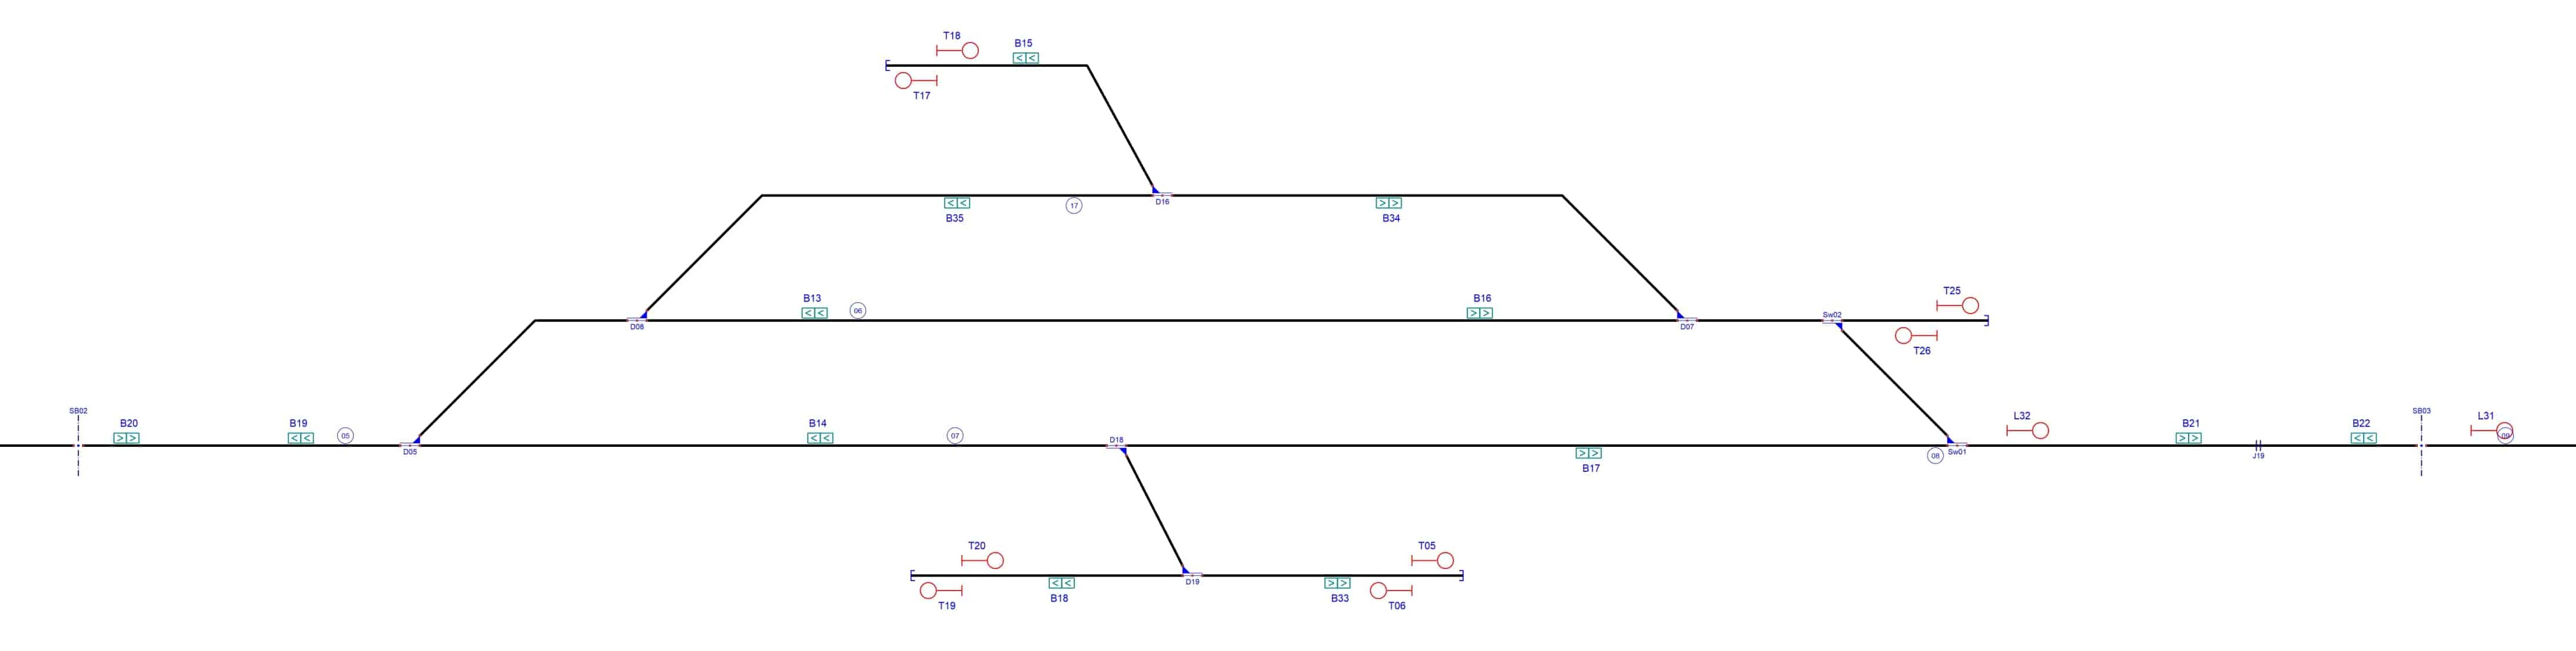
\includegraphics[width=1\textwidth]{resultados-obtenidos/ejemplo4/images/4_step1.png}
	\centering\caption{Señalamiento generado por el RNA para proteger el fin de vía.}
	\label{fig:EJ4_3}
\end{figure}

Los finales de vías absolutos son protegidos por las señales de parada T01, T03, T05, T07, T09, T11, T13, T15, T17, T19, T21, T23, T25 y T27; y las señales de partida son T02, T04, T06, T08, T10, T12, T14, T16, T18, T20, T22, T24, T26 y T28. A su vez, al no existir finales de vías relativos, el RNA no les asignó señales específicas.

La Figura \ref{fig:EJ4_4} ilustra la generación de señales destinadas a proteger las junturas entre los rieles. Las señales generadas son todas las señales entre J34 y J49, indicadas en color rojo. De no existir junturas que proteger, el RNA salteará este paso.

\begin{figure}[H]
	\centering
	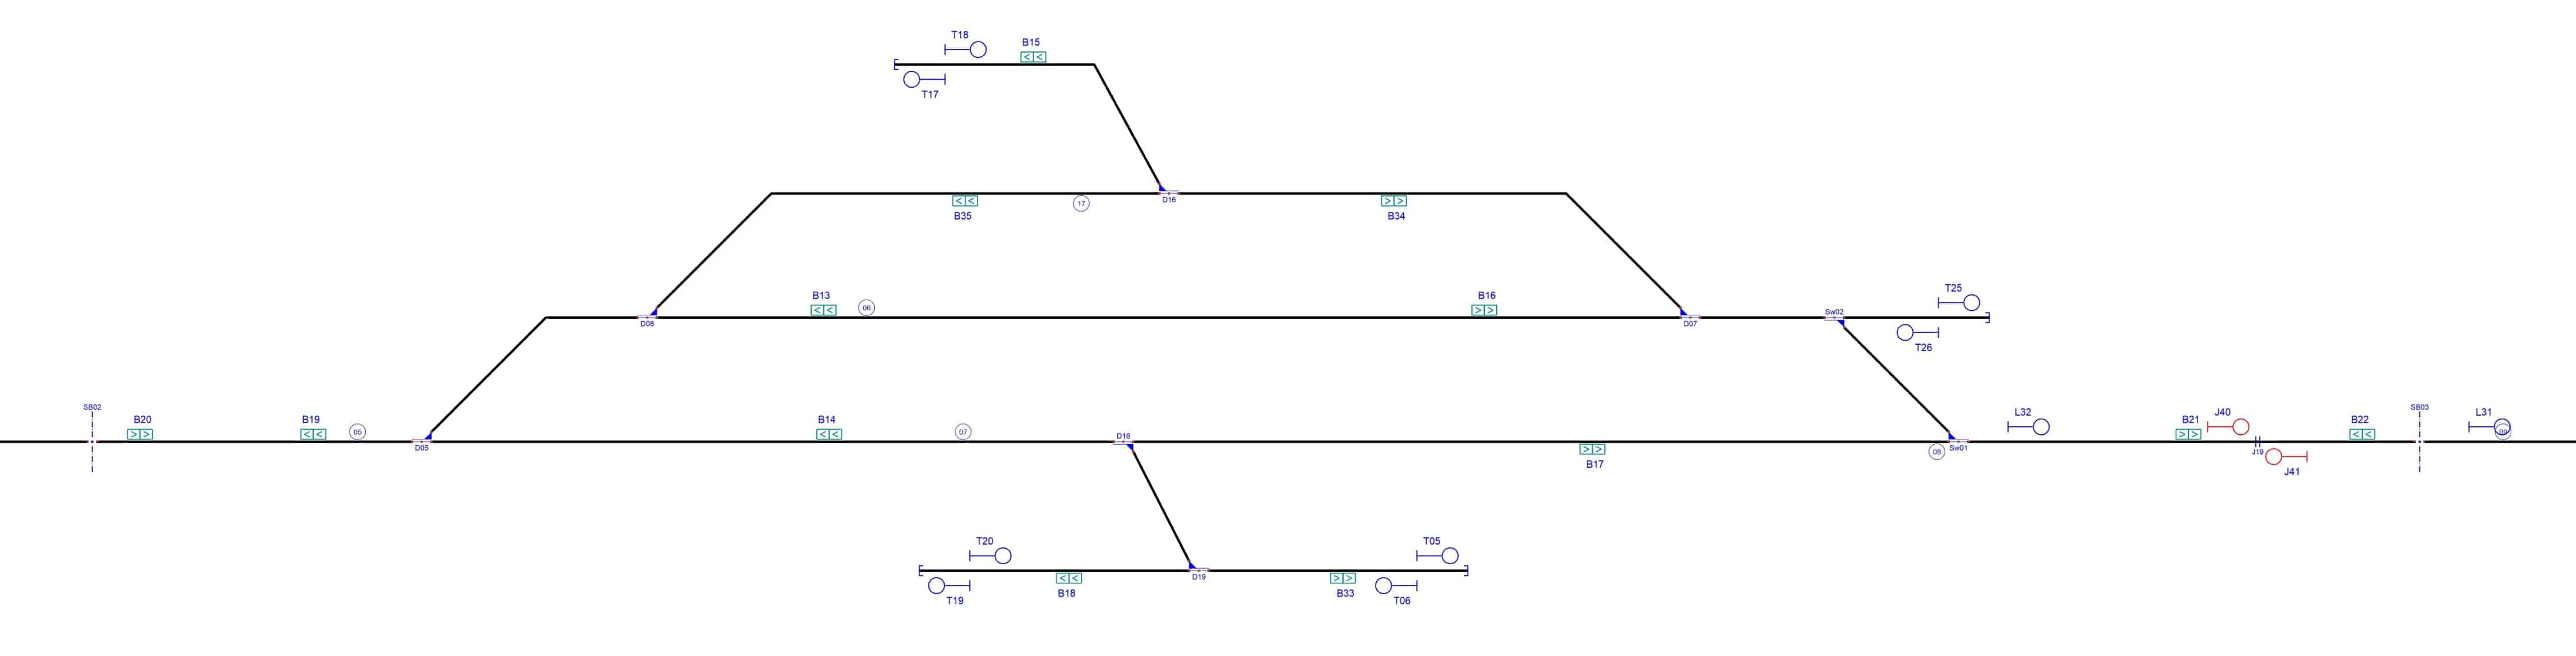
\includegraphics[width=1\textwidth]{resultados-obtenidos/ejemplo4/images/4_step2.png}
	\centering\caption{Señalamiento generado por el RNA para proteger las junturas.}
	\label{fig:EJ4_4}
\end{figure}

Al generar el señalamiento para proteger la infraestructura, tal como se explicó en la Sección \ref{sec:horizontal}, el Algoritmo \ref{alg:horizontal} simplificará las señales entre dos elementos ferroviarios si no existe espacio suficiente entre ellos. El señalamiento generado para proteger las plataformas y los cruces de vía se ilustra en rojo en la Figura \ref{fig:EJ4_5}. No se asignaron señales para proteger las plataformas, al no existir en este ejemplo. Por otro lado, las señales que protegen los cruces de vía son las señales comprendidas entre X50 y X53.

\begin{figure}[H]
	\centering
	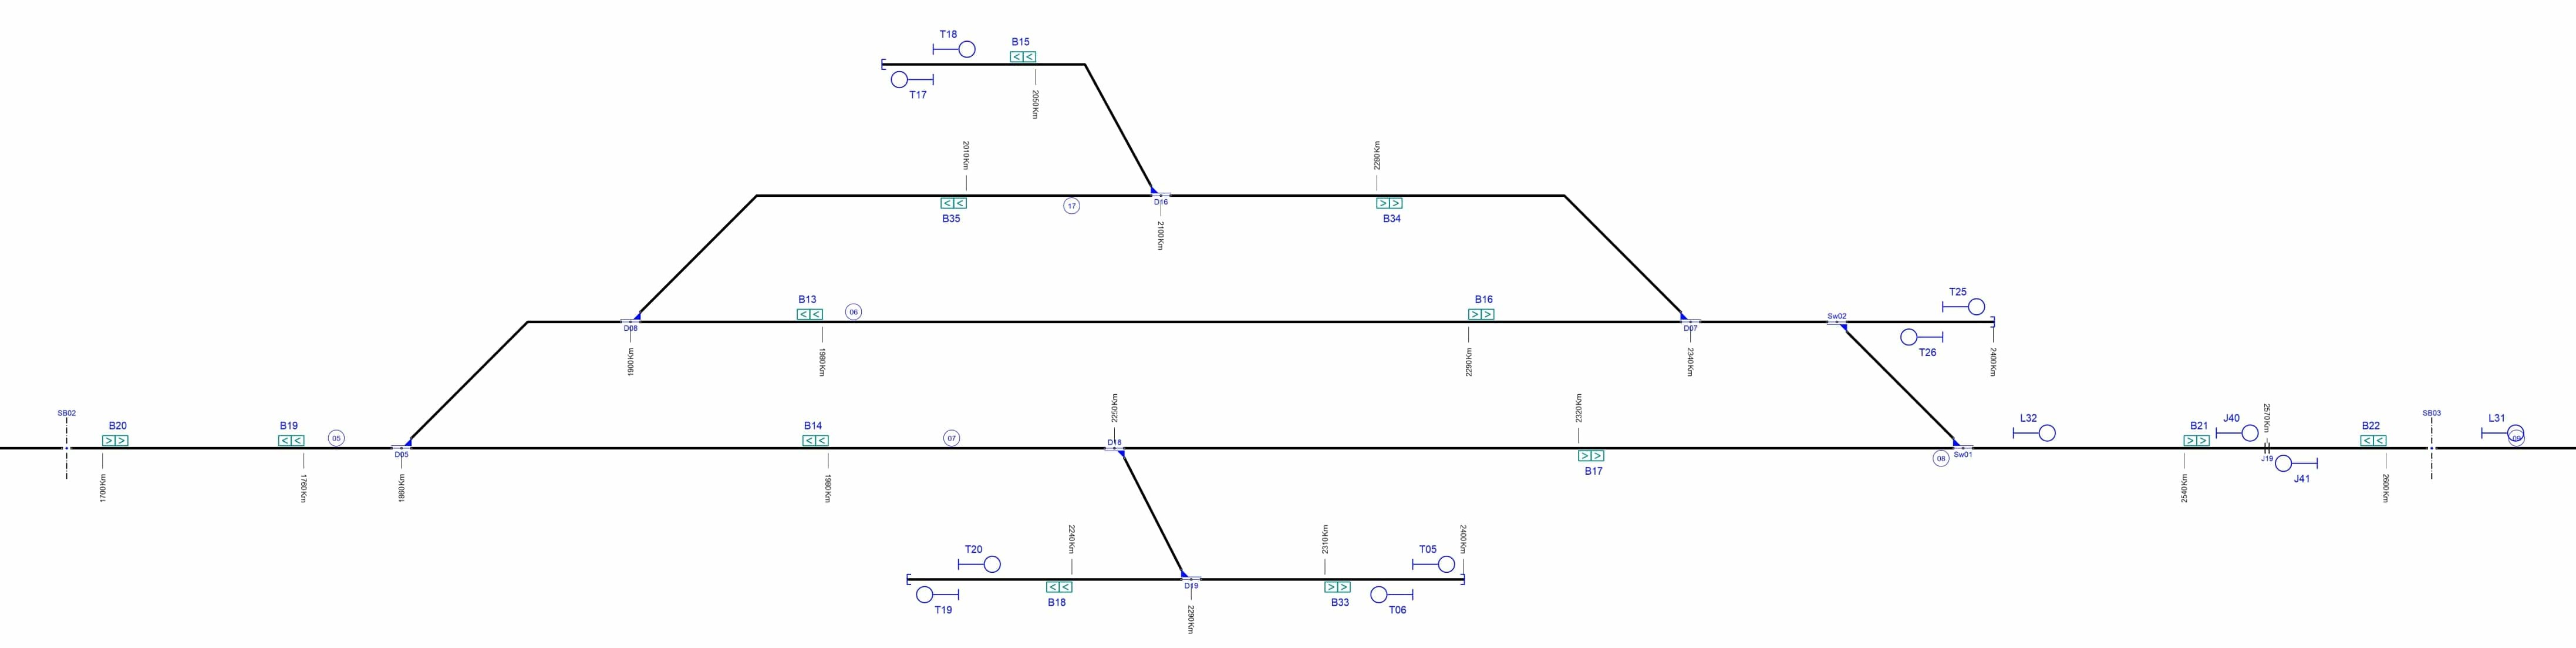
\includegraphics[width=1\textwidth]{resultados-obtenidos/ejemplo4/images/4_step3.png}
	\centering\caption{Señalamiento generado por el RNA para proteger plataformas y cruces de vía.}
	\label{fig:EJ4_5}
\end{figure}

El RNA generó 75 señales para proteger cada uno de los cambio de vías. Estas señales se encuentran resaltadas en rojo en la Figura \ref{fig:EJ4_6}.

\begin{figure}[H]
	\centering
	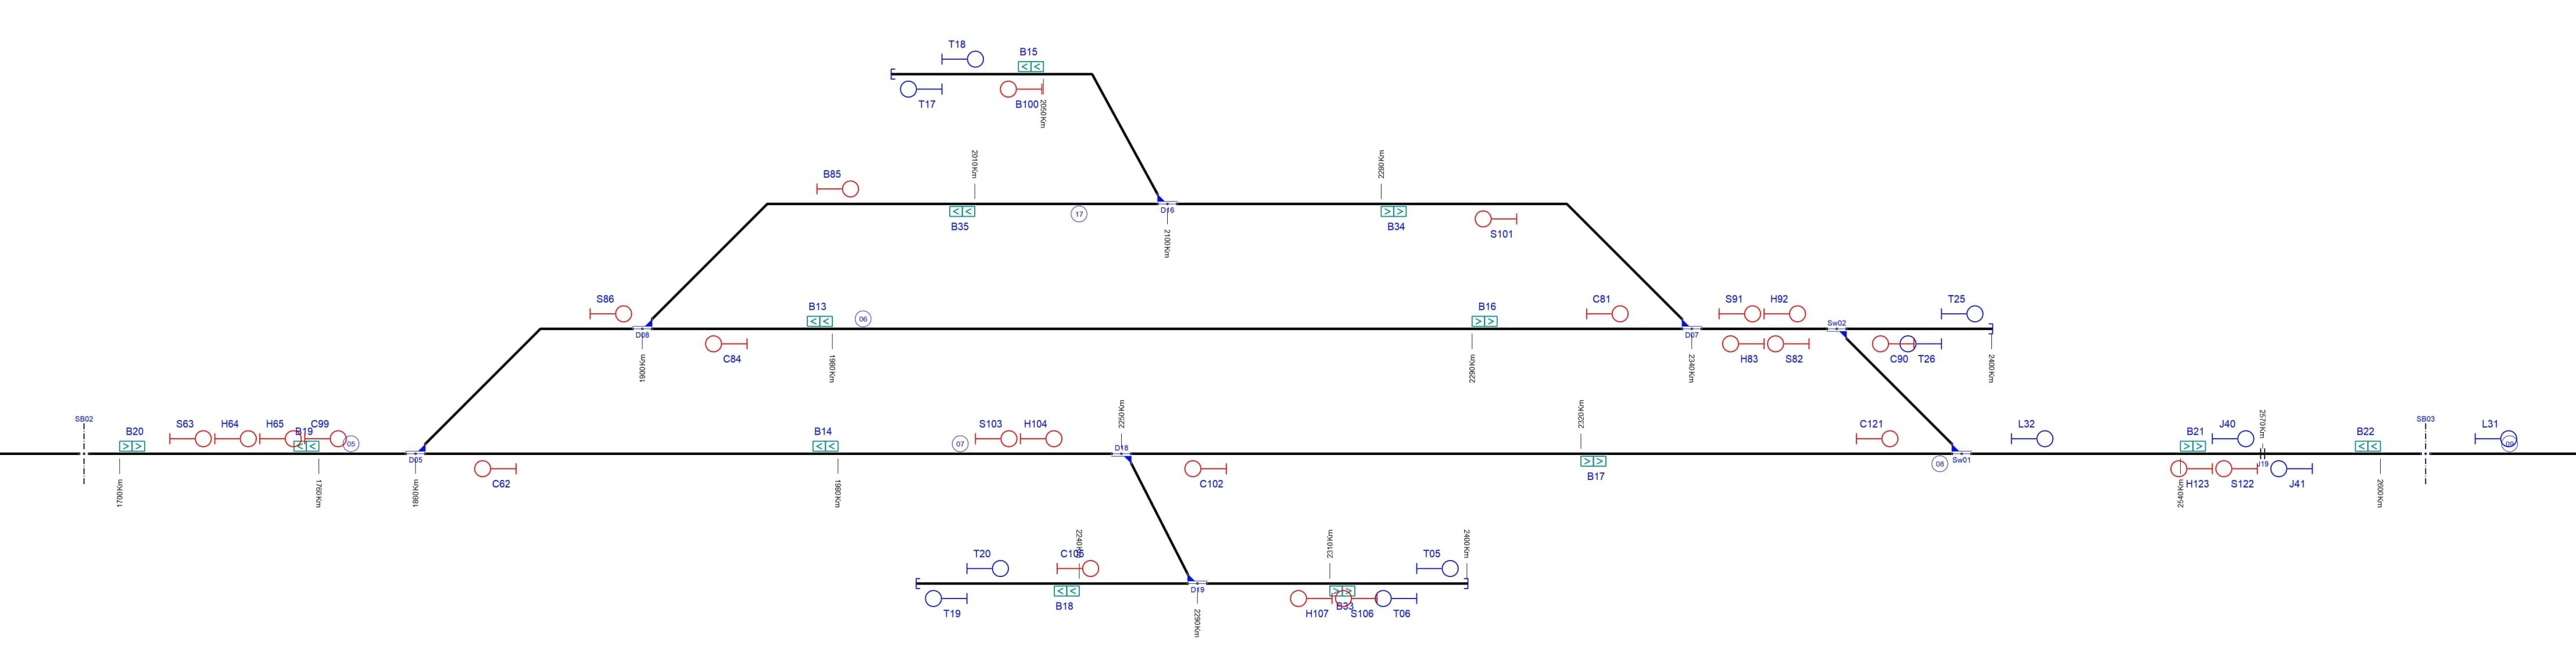
\includegraphics[width=1\textwidth]{resultados-obtenidos/ejemplo4/images/4_step4.png}
	\centering\caption{Señalamiento generado por el RNA para proteger los cambios de vías.}
	\label{fig:EJ4_6}
\end{figure}

Una vez obtenido todo el señalamiento, el RNA procede a simplificar las señales redundantes, repetidas o cuyas funciones o ubicaciones se superponen entre sí. El proceso de simplificación de señales fue explicado en la Sección \ref{sec:simplificacion}. El Algoritmo \ref{alg:vertical} de herencia vertical fue aplicado en las señales B entre los cambios de vías que comparan al menos una rama secundaria, desplazando las señales hasta convertirlas en las señales de herencia en las ramas principales. A continuación, se aplicó el Algoritmo \ref{alg:horizontal}, diseñado para agrupar objetos cercanos como un único objeto, generando el señalamiento acorde a los elementos contenidos en cada extremo del nuevo elemento contenedor.

Finalmente, las señales son simplificadas aplicando el Algoritmo \ref{alg:reduction} de eliminación por prioridad de señales. El resultado de este proceso es detallado en el Código \ref{lst:EJ4_3}.

\begin{lstlisting}[language = {}, tabsize=4, basicstyle=\footnotesize\ttfamily, showspaces=false, showstringspaces=false, caption = Reducción de señalamiento por prioridad de señales, label = {lst:EJ4_3}]
	Reducing redundant signals
	removing sig97 for sig04
	removing sig98 for sig04
	removing sig106 for sig06
	removing sig107 for sig06
	removing sig115 for sig10
	removing sig116 for sig10
	removing sig96 for sig16
	removing sig100 for sig17
	removing sig105 for sig20
	removing sig114 for sig22
	removing sig118 for sig23
	removing sig90 for sig26
	removing sig124 for sig28
	removing sig32 for sig40
	removing sig33 for sig38
	removing sig34 for sig94
	removing sig70 for sig35
	removing sig127 for sig36
	removing sig93 for sig37
	removing sig39 for sig128
	removing sig41 for sig122
	removing sig42 for sig67
	removing sig44 for sig112
	removing sig66 for sig45
	removing sig108 for sig46
	removing sig111 for sig47
	removing sig49 for sig109
	removing sig50 for sig52
	removing sig51 for sig53
	removing sig54 for sig58
	removing sig55 for sig59
	removing sig56 for sig60
	removing sig57 for sig61
	removing sig99 for sig63
	removing sig64 for sig63
	removing sig65 for sig63
	removing sig117 for sig67
	removing sig68 for sig67
	removing sig69 for sig67
	removing sig72 for sig71
	removing sig73 for sig71
	removing sig80 for sig79
	removing sig83 for sig82
	removing sig92 for sig91
	removing sig95 for sig94
	removing sig104 for sig103
	removing sig110 for sig109
	removing sig113 for sig112
	removing sig120 for sig119
	removing sig123 for sig122
	removing sig126 for sig125
	removing sig129 for sig128
\end{lstlisting}

	El resultado de la simplificación del señalamiento se ilustra en la Figura \ref{fig:EJ4_7}.
	
	\begin{figure}[H]
		\centering
		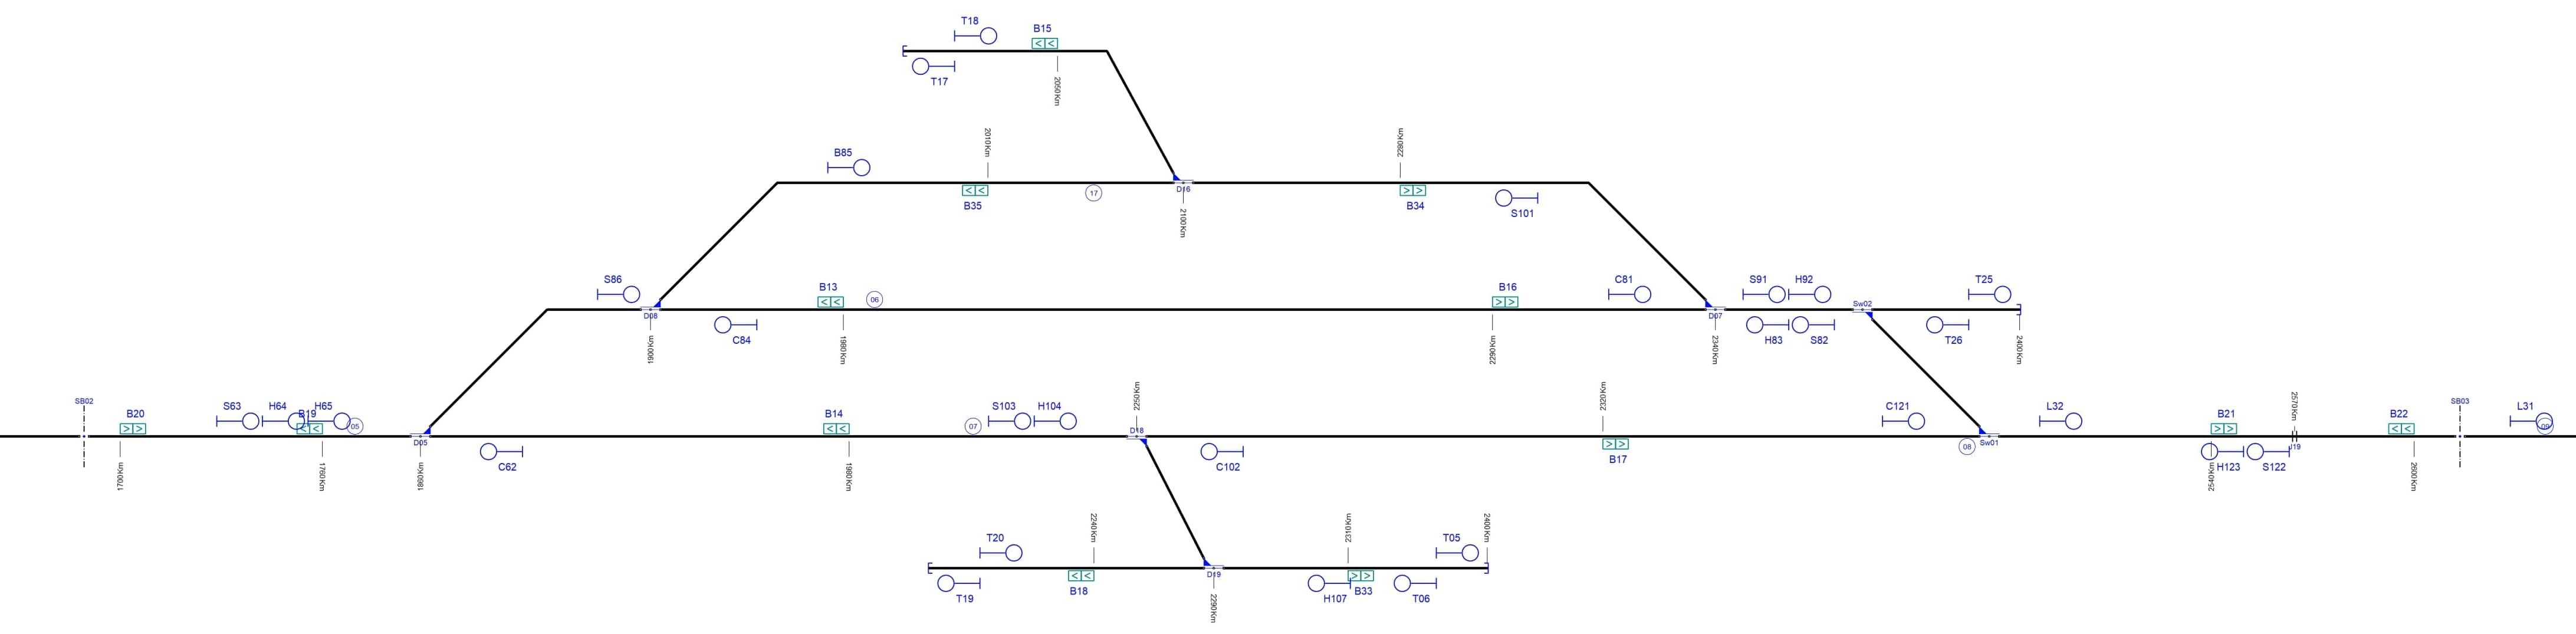
\includegraphics[width=1\textwidth]{resultados-obtenidos/ejemplo4/images/4_RNA.png}
		\centering\caption{Señalamiento generado y simplificado por el RNA.}
		\label{fig:EJ4_7}
	\end{figure}
	
	Al finalizar la generación del señalamiento, el RNA debe detectar todas las posibles rutas admitidas por la red para crear la tabla de enclavamientos. El RNA exporta los resultados del análisis en los siguientes cuatro documentos: Infrastructure.RNA (Apéndice \ref{sec:infrastructureRNA}), SafePoint.RNA (Apéndice \ref{sec:safePointsRNA}), Signalling.RNA (Apéndice \ref{sec:signallingRNA}) y Routes.RNA (Apéndice \ref{sec:routesRNA}).